\documentclass[sigconf]{acmart}

\usepackage{booktabs} % For formal tables


% Copyright
%\setcopyright{none}
%\setcopyright{acmcopyright}
%\setcopyright{acmlicensed}
\setcopyright{rightsretained}
%\setcopyright{usgov}
%\setcopyright{usgovmixed}
%\setcopyright{cagov}
%\setcopyright{cagovmixed}


% DOI
\acmDOI{10.475/123_4}

% ISBN
\acmISBN{123-4567-24-567/08/06}

%Conference
\acmConference[CODASPY'18]{ACM SDN-NFV Security 2018}{March 2018}{Tempe, Arizona, USA} 
\acmYear{1997}
\copyrightyear{2016}


\acmArticle{4}
\acmPrice{15.00}

% These commands are optional
%\acmBooktitle{Transactions of the ACM Woodstock conference}
\editor{Jennifer B. Sartor}
\editor{Theo D'Hondt}
\editor{Wolfgang De Meuter}


\begin{document}
\title{Feasibility Study of SDN-Firewalls : Design Vulnerabilities and Mitigation Techniques}
\titlenote{Produces the permission block, and
  copyright information}
%\subtitle{Extended Abstract}
%\subtitlenote{The full version of the author's guide is available as
%  \texttt{acmart.pdf} document}

\begin{comment}
\author{Ben Trovato}
\authornote{Dr.~Trovato insisted his name be first.}
\orcid{1234-5678-9012}
\affiliation{%
  \institution{Institute for Clarity in Documentation}
  \streetaddress{P.O. Box 1212}
  \city{Dublin} 
  \state{Ohio} 
  \postcode{43017-6221}
}
\email{trovato@corporation.com}

\author{G.K.M. Tobin}
\authornote{The secretary disavows any knowledge of this author's actions.}
\affiliation{%
  \institution{Institute for Clarity in Documentation}
  \streetaddress{P.O. Box 1212}
  \city{Dublin} 
  \state{Ohio} 
  \postcode{43017-6221}
}
\email{webmaster@marysville-ohio.com}

\author{Lars Th{\o}rv{\"a}ld}
\authornote{This author is the
  one who did all the really hard work.}
\affiliation{%
  \institution{The Th{\o}rv{\"a}ld Group}
  \streetaddress{1 Th{\o}rv{\"a}ld Circle}
  \city{Hekla} 
  \country{Iceland}}
\email{larst@affiliation.org}

% The default list of authors is too long for headers.
\renewcommand{\shortauthors}{B. Trovato et al.}
\end{comment}

\begin{abstract}
	Software-Defined Networking (SDN) is a novel approach towards network programmability. It provides physical separation of a control plane and forwarding plane. The SDN controller maintains the centralized view of the network and provides the ability to program the forwarding plane. However, the SDN network architecture has been prone to several security vulnerabilities since its very inception. At the same time, SDN Controllers and the its protocols are rapidly changing to address the scaling demands of complex enterprise networks. However, the rate at which SDN framework has been evolving remains unmatched by the advancements to address its security issues. \\ 
	According to our study, existing defense mechanisms are obsolete or incomplete to defend the latest SDN infrastructure. SDN firewalls in particular lack measures to provide robust security against attacks originating from outside and within the network. This paper surveys existing SDN firewall designs and their shortcomings to protect advanced controllers and protocol. By testing these solutions on the production size of a network, new attack vectors have been discovered. Corresponding threat detection techniques and respective mitigation strategies are also proposed.
	\footnote{This is an abstract footnote}
\end{abstract}

%
% The code below should be generated by the tool at
% http://dl.acm.org/ccs.cfm
% Please copy and paste the code instead of the example below. 
%
\begin{CCSXML}
<ccs2012>
 <concept>
  <concept_id>10010520.10010553.10010562</concept_id>
  <concept_desc>Computer systems organization~Embedded systems</concept_desc>
  <concept_significance>500</concept_significance>
 </concept>
 <concept>
  <concept_id>10010520.10010575.10010755</concept_id>
  <concept_desc>Computer systems organization~Redundancy</concept_desc>
  <concept_significance>300</concept_significance>
 </concept>
 <concept>
  <concept_id>10010520.10010553.10010554</concept_id>
  <concept_desc>Computer systems organization~Robotics</concept_desc>
  <concept_significance>100</concept_significance>
 </concept>
 <concept>
  <concept_id>10003033.10003083.10003095</concept_id>
  <concept_desc>Networks~Network reliability</concept_desc>
  <concept_significance>100</concept_significance>
 </concept>
</ccs2012>  
\end{CCSXML}

\ccsdesc[500]{Computer systems organization~Network properties}
\ccsdesc[300]{Network Security}
\ccsdesc[100]{Firewalls}


\keywords{Software Defined Networking (SDN), Network Security, OpenFlow}


\maketitle

\section{Introduction}

Software-Defined Networking is a new network paradigm which has greatly
changed the operating procedures of a network when compared to traditional
networks. A traditional network uses a set of devices like router and 
switches to provide connectivity to the entire network. A set of forwarding rules
in these devices decide and direct the flow of a network traffic. A network 
admin generally is responsible to program and maintain these forwarding 
rules individually in all the switches and routers. The control plane on a device
keeps track of the forwarding logic and the forwarding plane\footnote
{Also called Data Plane} does as instructed by the control plane. 
Software-Defined Networking has brought significant change as networks function by
decoupling the entire control plane from the forwarding plane. Abstraction of higher level functionality is achieved and the intelligence of a 
network  ia now moved to a centralized location called SDN-Controller. 
Central programmability and visibility have brought tremendous
improvements in operational and maintenance costs of networks.

This paradigm shift has influenced both industries and academic institutions to 
persistently work towards SDN networks. The strong push of cost effective scalable 
networks has lead to transformation of traditional networks and
deployment of SDN infrastructure in production networks like Data-Centers and enterprise Clouds. The merits of SDN has also made it increasingly becoming popular in academic institutions as well.
The campus networks today generate tremendous amount of data making data intensive science a common norm.
To appropriately handle the data without significant loss in information, the campus networks have begin to 
dedicate a portion of the network model for advanced research operations on the traffic.

This new model termed as Science-DMZ, is a SDN solution specifically designed for optimizing network transaction 
on academic networks. The model allows the existing tools and methods to be optimized for protecting science critical systems.
Science-DMZ network is often built around the campus' local network perimeter. To employ a belt of security in this perimeter network,
institutions often depend on legacy firewalls and Intrusion Detection Systems. Both of these security mechanisms are ill-suited 
for protecting SDN environments. The traditional Firewalls function based on a static rule set consisting of ALLOW and DENY policies. The filtering
of network traffic is done by matching each packet against the rules. The most granular rules can match a packet against only source and destination IP addresses and TCP/UDP ports. These kind of rules cannot be further fine grained and lack adaptivity and scalability. The SDN-Firewall solution is thus required which can work closely with the controller and take advantage of the centralized view.

Some related work has been done in the recent past to address security concerns specific to SDN networks. There exist SDN specific firewalls
which work in collaboration with the SDN-Controller to provide centralized security solution. Present firewall solutions are often presented as a prototype to work well on small-scale controllers and old protocol versions. Additionally,they often employ standard network simulation techniques for testing. They, however, fail to adapt for meeting rapidly changing SDN controllers' design and revisions in OpenFlow protocol. Thus, there lies inherent need of revisiting the SDN firewalls to find the shortcomings and the new vulnerabilities that might appear on a more real-time and large-scale networks.

In this paper, we have revisited the existing SDN firewall designs and attempted to deploy these works on Science-DMZ network to discover realtime challenges.
In our testbed, we have incorporated mainstream SDN controller, OpenDayLight and OpenFlow protocol 1.3, both of which are actively in use on many enterprise networks. Our experiments show that proposed approaches to detect policy violations are prone to security loopholes that urgently need to get addressed for a promised SDN security. It is also discovered that the defense and attack mitigation models are obsolete and incomplete to safeguard a larger network with changed controller design. The new vulnerabilities found in existing solutions are investigated and suitable defense mechanisms are also proposed. The performance of present SDN firewalls was tested in simulated environments, leading to wariness of their feasibility in an enterprise network.
We have measured the operating performance of existing defense mechanisms on Science-DMZ network and have realized a room for improvement. An optimized approach to detect security policy violations has been devised and presented with improved results.

\section{SDN Background}
\subsection{Openflow}
Software-Defined Networking has decoupled the control plane logic from the switches and moved the forwarding decision and policy enforcement capability to the Controller. Communications between SDN logical abstractions is achieved by using different protocols depending on the layers wanting to communicate. Interaction between SDN-Controller and switches happens by provisioning APIs of a southbound protocol called OpenFlow.
Controller leverages OpenFlow protocol to pull the information from switches and feed the forwarding logic back. OpenFlow enabled switches maintain the flow routing policies in flow tables. A typical flow rules present in flow table has 3 different fields for packet handling: Match, Action and Flow statistics. The match field allows packet filtering based on layer 1-4 header fields. The rules are matched based on priorities and after a successful match the packet undergoes respective action present in the flow rule. First packet of every traffic flow is typically sent to controller and controller then inspects the packet headers to decide the action to be taken for the flow. These actions can be either DROP or FORWARD. An SDN Controller can potentially enforce the centrally enforced security policies and take a suitable action for every packet that is received by it. The central visibility is of great advantage as control can easily extrapolate the future impact of allowing or denying such a traffic in the network on any other node in the network.

\subsection{Controller Design}
SDN-Controllers are capable of a lot more than a traditional control plane where the node os oblivious of the network activity in any other node in the network. There are different SDN controllers in the market. Some light weighted ones are used for academic testing and prototyping. The enterprise-ready controllers, however are complicated in their design and functioning. Thus, due to lack of implementation standards, these controllers are implemented differently and often leave security loopholes in their implementation and design. Two of the most widely recognized SDN controllers in the market are OpenDayLight \footnote{Henceforth, referred as ODL} and Open Network Operating System\footnote{Henceforth, referred as ONOS}, both are open-source projects hosted by The Linux Foundation. They both differ greatly in their designs. 

\subsubsection{OpenDaylight}
OpenDayLight is a SDN controller based on Model-View-Control platform written in Java. ODL provides several controller services implemented as part of it's kernel and Service Abstraction Layer, MD-SAL. Some of the major services running in ODL include L2switch, OpenflowPlugin and MD-SAL. To operate concurrently, these services take data from a common information storehouse present within the ODL core architecture. To store the data coming from northbound REST APIs and from southbound OpenFlow protocol, ODL, implements two logical datastores. Operational store contains the active and opearting state of the network, the information is directly retrieved from the network. Config store, however, contains information as the applications operating on controller and the network administrator intends. This is different from operational store in which it does not retrieve the information from the network. Instead, it contains information  that is directly fed to it using REST APIs and also programmaticaly from services like firewall running inside or outside controller.
Consequently, the administrator or a Firewall application can only make GET requests from the operational datastore. But, the CONFIG datastore provides GET, PUT, POST and DELETE procedural transactions for playing with data. An SDN firewall typically makes GET information to retrieve the latest flow rules and topology of the network. CONFIG store is used by a firewall to put the counter measures and to modify the existing OpenFlow rules. Finally, ODL discourages use of external databases for the performance reasons and leverages its in-memory datastores based on XSQL. 

\subsubsection{Open Network Operating System}

ONOS is being marketed as a SDN Operating System rather than as a controller. Different subsystems on ONOS gives the modularity and high level of service abstraction. Common subsystems on ONOS include Device, Link and FlowRule subsystems. The datastores here are divided in two categories: services running on controller have separate datastore per service and each device present in the network has a datastore of its own. Device and topology information is stored in Device Config Store, implemented using distributed Doctree model. The services like firewall get a separate Service Config Store. Applications can initiate the transfer of config parameters from service to device config store. Device drivers ultimately then program the switches present in the topology.  

\subsection{Firewalls}

A conventional firewall is a system that protects the trusted internal network from the untrusted and unsecured outside network, such as Internet.
Firewalls filters and scan the traffic in and out of the network. Layer-3 and Layer-4 header fields from a traffic flow is compared against a static set of security policies, such as ACLs. In a paradigm of SDN, the positioning, functioning and capabilities of a firewall witness multiple adaptations. SDN architecture allows the network to be managed centrally, deeming the forwarding plane to be a set of vacuous boxes. Thus, the firewall logic should be placed on a control plane alongside, SDN-Controller. SDN-firewall having a centralized view of a network, can additionally inspect local traffic to detect internal policy violations and network reachability. The firewall policies are centrally enforced at the controller and a software application is responsible for installing filtering rules on the network. 
Unlike traditional firewall which filters and scans every packet coming and going through it, an SDN-Firewall gets the first packet of each flow and install flow rule policies for the rest of the flow in flow tables of respective switches. Flows can directly be installed by an administrator and a privileged application in controller. SDN-firewall should check for policy enforcement by verifying the impact of such changes in the network before a violation can potentially happen. 

Additionally, an SDN firewall works on an abstracted design of network. This is different from a traditional firewall. Thus, SDN-Firewall should check for any threats that can originate from northbound and southbound communication.
 
\begin{figure}
	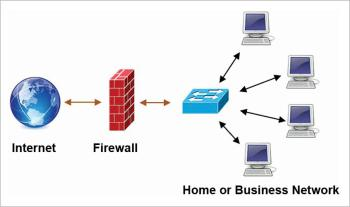
\includegraphics[height=2in, width=2in]{traditional}
	\caption{ Firewall in  \texttt{traditional} network}
	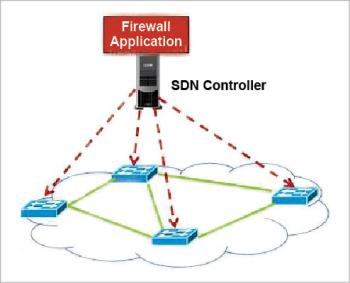
\includegraphics[height=2in, width=2in]{SDN-Firewall}
	\caption{ Firewall in  \texttt{SDN} network}
\end{figure}   

\section{Survey of {\itshape obsolete} SDN-Firewalls}

FlowGuard is an SDN-Firewall prototype solution built on FloodLight controller and OpenFlow 1.1. To  detect flow policy violations, FlowGuard pulls the network topology and flow rules from the data plane. It has leveraged Header Spavce analysis and NetPlumber library to build a plumbing graph. This graph is used as a logical snapshot of the network. A flow path space is a tracked space of a packet in the network comprising of initial source and final destination addresses. The flow path space calculation is based on IP 5-Tuple sense: source, destination IP and ports with protocol. Further, comparing the flow path space against the Firewall DENY rules, FlowGuard detects any security policy violations.

\subsection{Flow Path Space} Upon testing the firewall on ODL controller and on a complicated topology, it was found that the IP-5 Tuple based approach is prone to ambiguous flow path calculations. An SND-Firewall with a centralized view of two or more different tenants, cannot successfully distinguish between tenants based solely on IP 5-Tuples. In a tenant based network like in datacenter, multiple disconnected tenants can be using DHCP servers with similar configurations. This will lead to hosts having similar IP 5-tuple addresses in two disconnected tenants. Upon testing FlowGuard on an Openstack cloud with multiple different tenants, Flowguard produced conflicting flow path spaces and the comparison against the Firewall rules gave confusing results. 
% Check for more concrete example, where with 5-tuple, firewall gives error.

In order to prevent the conflict, a more fine grained, Openflow 10-Tuple sense should rather be used. Apart from the exisitng fields in IP 5-Tuple sense, an OpenFlow 10-tuple also includes a physical layer-2  port, protocol type, VLAN-ID and Ethernet type. With these header fields, it is impossible to have duplicate route identification and thus prevent the ambiguity in flow path space calculation. 

\subsection{Firewall rule priority}

In a conventional firewall, priority of the rules are implicit based on their ordering. Provided a successful match, only higher priority firewall rule is considered for the action on traffic. In an SDN-firewall, the firewall rules and flow rules maintain their own set of priorities. SDN-Firewalls like FlowGuard, divides the firewall rule space into two disjoint sets of \textit{allow} and \textit{deny} rules. These partitioning is however either done considering implicit rule priorities like in IP-tables or not considered at all. Thus, the firewall decision logic may violate the administrators intent of policy enforcement.

This can be fixed by taking the priorities of policies in account. However, this appears to be a difficult problem, as there are multiple sources like IDS, feedback module, firewall and network administrator can potentially install policies ignorant of what higher priority conflicting rules exist in the network. It is still a problem when their are no action-based conflicts between the rules, as redundant rules take unnecessary disk apce on the controller. Duplicate rules are also a cause of performance degradation while checking for policy violations in the network. 
% Work on the dynamic priority decision algorithm

\subsection{Violation Resolution approaches}
 Upon successful detection of flow and firewall policy violations, an SDN-Firewall should also be able to dynamically resolve the violations by either denying the new rules or modifying the existing flow tables. There are different approaches in place to mitigate various kinds of violations. Many of these proposed approaches do their job of removing the violations but at the cost of availability and accuracy: deleted, modified and new rules prevent unauthorized traffic in the network by also denying communication between authorized hosts.
	\subsubsection{Approach 1}
 	 Dependency between flow rules having set-field actions can cause traffic to be matched by an unwanted flow rule. This can cause traffic steering among unauthorized hosts as mentioned in FlowGuard. A novel approach to break the inter-dependency is by using tags. Match fields in flow rules are tagged to break any violating dependencies. This is however achieved at the cost of losing the critical information of the flow field which is tagged. For eg., in FlowGuard, vlan-tagging is used wherein VLAN field in flow rule is tagged to break its dependency from another flow rule in same or different switch. In our testing in multi tenant networks, VLAN field plays a significant role in traffic steering between different subnets. Thus, by tagging VLAN field with a hard coded value, the dependency can be broken but the flow rules intended purpose to match on VLAN field is lost. Also, any flows which were not part of dependency process but were using the tagged field to process the pcket further in the network, fail to match the traffic in which packet headers are now changed. 
	\subsubsection{Approach 2}
 	 When a firewall detects there is entire violation in the existing flow path, all the rules present in the flow path are removed from the corresponding switches on the network. Only tracked path comprising of source address from the incoming packets and destination address from the outgoing packet is matched against the Firewall rule policies. In our testing we found that this approach leaves the netowork disconnected if the  \textit{tracked flow path space} encompasses more than two switches or flow tables. For eg., if a violating tracked space consists of rules from 5 different switches and one of the rules in the third switch(middle node) is a wildcarded rule allowing this "unauthorized" communication, all the rules including the wildcared one are deemed unnecessary and removed. This further leads to denial of any authorized communication also that the wildcarded rule was allowing in the network.
 	 % Give the example in diagram
 	 To prevent such complex resolutions from being too hard on the network, higher priority rules with finer granularity should be added. The wildcarded flows require special attention as they are responsible for both allowed and denied traffic through them.
	\subsubsection{Approach 3}
	 Another issue with removing a flow from a network is that with new Openflow protocol, the actions per match in a flow rule can be chained. This means, when a flow in netowrk is matched by a flow rule in a switch, the same packet can undergo multiple actions, which include output to a physical port of that switch, send to controller or DROP. Upon detecting a violation in a flow rule, deleting the entire flow rule, deletes all the violating and non violating actions within it. This means the deletion of a flow rule requires carefully examination. The action set within a rule can only partialy violate the policy just like entire flow rule can have partial violations.

 \subsection{Disregard for concurrent updates}
 In our testing we have found issues when multiple user threads or applications make concurrent updates on firewall policy or flow policy. In case of conflicting updates, lack of handling the concurrency leads to low priority rule with a different action on same match being handled before the higher priority rule. For eg. if an admin uses REST call to install a new flow rule in the network but a countermeasure engine at the same time install a conflicting action on the same match as by REST call, the decision of unsynchronized firewall depends on which thread is executed before. The issue with concurrent updates becomes a problem when firewall applications are deployed in an enterprise networks where there are multiple pipelines which update the same flow policy data stores.
 
\section{Advanced SDN-Firewall}
The attacks in a complex network like datacenters can originate from external world and from within. As mentioned before, the SDN-firewall cannot trust the traffic and hosts present inside the network just like the outside world. The existing firewall solutions customized for SDN network keep a check on internal traffic. However, the approach is merely an implementation of Access Control List model. The flow propagation is checked between the authorized and unauthorized hosts. Using the pool of information provided by OpenFlow protocol and SDN control plane, an SDN-Firewall potentially can provide multi dimension protection instead of just being a ACL policy enforcer. 

With abstraction in SDN layers in place, the attack can originate from not just outside the network, but from in
Discuss new attacks and strategies here. Tell that firewall in SND should be more than policy violation detection and resolution tool. It should also be able to check attacks like DoS, MITM, Flow flooding and other attacks. Ask professors whether this should actually be included as a part of a firewall(modern FW?) or in this paper.

Controller becomes unresponsive 
Flow installation time becomes super slow!!
Services regularly crash
DLUX does not respond to remote requests

END:
Flows were getting installed in CONFIG with 204 response code. But none were transferred to thenetwork. Cause is not known.

The OpenFlow protocol provides switch and flow metrics. This information is passed to controller using southbound APIs and can be fetched by application using REST calls from the north. We propose to extend the SDN-Firewall to do statistical analysis using the information from a network for anomaly detection.

\subsection{Attack Vectors}
A formula that appears in the running text is called an
inline or in-text formula.  It is produced by the
\textbf{math} environment, which can be
invoked with the usual \texttt{{\char'134}begin\,\ldots{\char'134}end}
construction or with the short form \texttt{\$\,\ldots\$}. You
can use any of the symbols and structures,
from $\alpha$ to $\omega$, available in
\LaTeX~\cite{Lamport:LaTeX}; this section will simply show a
few examples of in-text equations in context. Notice how
this equation:
\begin{math}
  \lim_{n\rightarrow \infty}x=0
\end{math},
set here in in-line math style, looks slightly different when
set in display style.  (See next section).

\subsection{Detection and mitigation}
A numbered display equation---one set off by vertical space from the
text and centered horizontally---is produced by the \textbf{equation}
environment. An unnumbered display equation is produced by the
\textbf{displaymath} environment.

Again, in either environment, you can use any of the symbols
and structures available in \LaTeX\@; this section will just
give a couple of examples of display equations in context.
First, consider the equation, shown as an inline equation above:
\begin{equation}
  \lim_{n\rightarrow \infty}x=0
\end{equation}
Notice how it is formatted somewhat differently in
the \textbf{displaymath}
environment.  Now, we'll enter an unnumbered equation:
\begin{displaymath}
  \sum_{i=0}^{\infty} x + 1
\end{displaymath}
and follow it with another numbered equation:
\begin{equation}
  \sum_{i=0}^{\infty}x_i=\int_{0}^{\pi+2} f
\end{equation}
just to demonstrate \LaTeX's able handling of numbering.

\subsection{Unfulfilled design requirements}
Citations to articles~\cite{bowman:reasoning,
clark:pct, braams:babel, herlihy:methodology},
conference proceedings~\cite{clark:pct} or maybe
books \cite{Lamport:LaTeX, salas:calculus} listed
in the Bibliography section of your
article will occur throughout the text of your article.
You should use BibTeX to automatically produce this bibliography;
you simply need to insert one of several citation commands with
a key of the item cited in the proper location in
the \texttt{.tex} file~\cite{Lamport:LaTeX}.
The key is a short reference you invent to uniquely
identify each work; in this sample document, the key is
the first author's surname and a
word from the title.  This identifying key is included
with each item in the \texttt{.bib} file for your article.

The details of the construction of the \texttt{.bib} file
are beyond the scope of this sample document, but more
information can be found in the \textit{Author's Guide},
and exhaustive details in the \textit{\LaTeX\ User's
Guide} by Lamport~\shortcite{Lamport:LaTeX}.

This article shows only the plainest form
of the citation command, using \texttt{{\char'134}cite}.

Some examples.  A paginated journal article \cite{Abril07}, an enumerated
journal article \cite{Cohen07}, a reference to an entire issue \cite{JCohen96},
a monograph (whole book) \cite{Kosiur01}, a monograph/whole book in a series (see 2a in spec. document)
\cite{Harel79}, a divisible-book such as an anthology or compilation \cite{Editor00}
followed by the same example, however we only output the series if the volume number is given
\cite{Editor00a} (so Editor00a's series should NOT be present since it has no vol. no.),
a chapter in a divisible book \cite{Spector90}, a chapter in a divisible book
in a series \cite{Douglass98}, a multi-volume work as book \cite{Knuth97},
an article in a proceedings (of a conference, symposium, workshop for example)
(paginated proceedings article) \cite{Andler79}, a proceedings article
with all possible elements \cite{Smith10}, an example of an enumerated
proceedings article \cite{VanGundy07},
an informally published work \cite{Harel78}, a doctoral dissertation \cite{Clarkson85},
a master's thesis: \cite{anisi03}, an online document / world wide web
resource \cite{Thornburg01, Ablamowicz07, Poker06}, a video game (Case 1) \cite{Obama08} and (Case 2) \cite{Novak03}
and \cite{Lee05} and (Case 3) a patent \cite{JoeScientist001},
work accepted for publication \cite{rous08}, 'YYYYb'-test for prolific author
\cite{SaeediMEJ10} and \cite{SaeediJETC10}. Other cites might contain
'duplicate' DOI and URLs (some SIAM articles) \cite{Kirschmer:2010:AEI:1958016.1958018}.
Boris / Barbara Beeton: multi-volume works as books
\cite{MR781536} and \cite{MR781537}.

A couple of citations with DOIs: \cite{2004:ITE:1009386.1010128,
  Kirschmer:2010:AEI:1958016.1958018}. 

Online citations: \cite{TUGInstmem, Thornburg01, CTANacmart}.  


\subsection{Proof of Concept SDN attacks}
Because tables cannot be split across pages, the best
placement for them is typically the top of the page
nearest their initial cite.  To
ensure this proper ``floating'' placement of tables, use the
environment \textbf{table} to enclose the table's contents and
the table caption.  The contents of the table itself must go
in the \textbf{tabular} environment, to
be aligned properly in rows and columns, with the desired
horizontal and vertical rules.  Again, detailed instructions
on \textbf{tabular} material
are found in the \textit{\LaTeX\ User's Guide}.

Immediately following this sentence is the point at which
Table~\ref{tab:freq} is included in the input file; compare the
placement of the table here with the table in the printed
output of this document.

\begin{table}
  \caption{Frequency of Special Characters}
  \label{tab:freq}
  \begin{tabular}{ccl}
    \toprule
    Non-English or Math&Frequency&Comments\\
    \midrule
    \O & 1 in 1,000& For Swedish names\\
    $\pi$ & 1 in 5& Common in math\\
    \$ & 4 in 5 & Used in business\\
    $\Psi^2_1$ & 1 in 40,000& Unexplained usage\\
  \bottomrule
\end{tabular}
\end{table}

To set a wider table, which takes up the whole width of the page's
live area, use the environment \textbf{table*} to enclose the table's
contents and the table caption.  As with a single-column table, this
wide table will ``float'' to a location deemed more desirable.
Immediately following this sentence is the point at which
Table~\ref{tab:commands} is included in the input file; again, it is
instructive to compare the placement of the table here with the table
in the printed output of this document.


\begin{table*}
  \caption{Some Typical Commands}
  \label{tab:commands}
  \begin{tabular}{ccl}
    \toprule
    Command &A Number & Comments\\
    \midrule
    \texttt{{\char'134}author} & 100& Author \\
    \texttt{{\char'134}table}& 300 & For tables\\
    \texttt{{\char'134}table*}& 400& For wider tables\\
    \bottomrule
  \end{tabular}
\end{table*}
% end the environment with {table*}, NOTE not {table}!

It is strongly recommended to use the package booktabs~\cite{Fear05}
and follow its main principles of typography with respect to tables:
\begin{enumerate}
\item Never, ever use vertical rules.
\item Never use double rules.
\end{enumerate}
It is also a good idea not to overuse horizontal rules.


\section{Implementaion and Evaluation}

Like tables, figures cannot be split across pages; the best placement
for them is typically the top or the bottom of the page nearest their
initial cite.  To ensure this proper ``floating'' placement of
figures, use the environment \textbf{figure} to enclose the figure and
its caption.

This sample document contains examples of \texttt{.eps} files to be
displayable with \LaTeX.  If you work with pdf\LaTeX, use files in the
\texttt{.pdf} format.  Note that most modern \TeX\ systems will convert
\texttt{.eps} to \texttt{.pdf} for you on the fly.  More details on
each of these are found in the \textit{Author's Guide}.

\begin{figure}
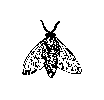
\includegraphics{fly}
\caption{A sample black and white graphic.}
\end{figure}

\begin{figure}
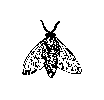
\includegraphics[height=1in, width=1in]{fly}
\caption{A sample black and white graphic
that has been resized with the \texttt{includegraphics} command.}
\end{figure}


As was the case with tables, you may want a figure that spans two
columns.  To do this, and still to ensure proper ``floating''
placement of tables, use the environment \textbf{figure*} to enclose
the figure and its caption.  And don't forget to end the environment
with \textbf{figure*}, not \textbf{figure}!

\begin{figure*}
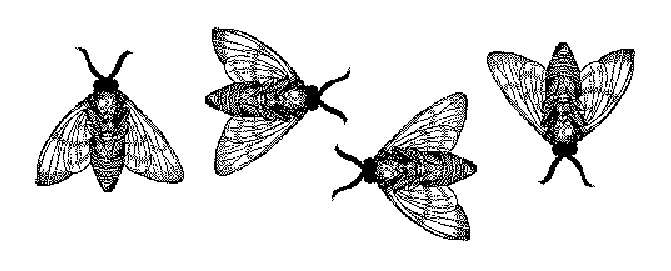
\includegraphics{flies}
\caption{A sample black and white graphic
that needs to span two columns of text.}
\end{figure*}


\begin{figure}
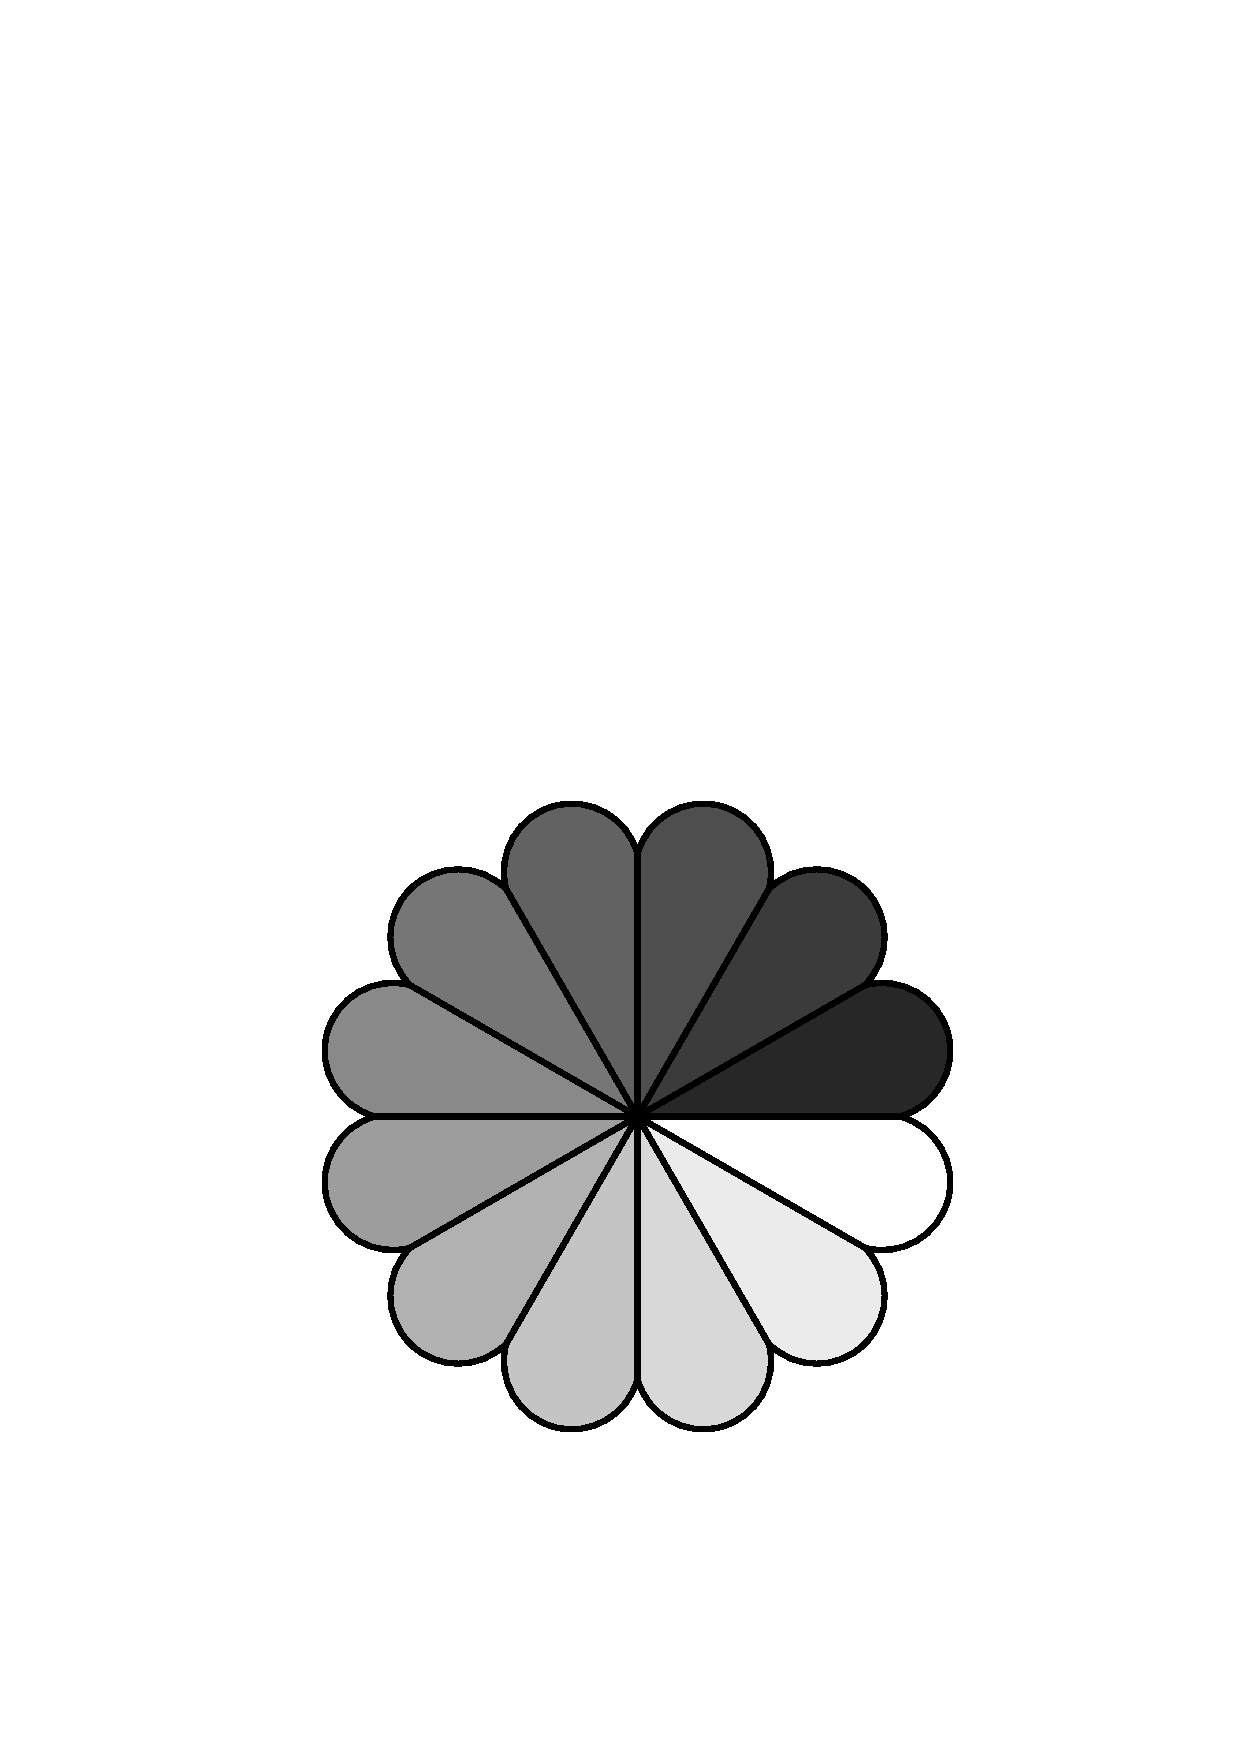
\includegraphics[height=1in, width=1in]{rosette}
\caption{A sample black and white graphic that has
been resized with the \texttt{includegraphics} command.}
\end{figure}

\section{Conclusion}

Other common constructs that may occur in your article are the forms
for logical constructs like theorems, axioms, corollaries and proofs.
ACM uses two types of these constructs:  theorem-like and
definition-like.

Here is a theorem:
\begin{theorem}
  Let $f$ be continuous on $[a,b]$.  If $G$ is
  an antiderivative for $f$ on $[a,b]$, then
  \begin{displaymath}
    \int^b_af(t)\,dt = G(b) - G(a).
  \end{displaymath}
\end{theorem}

Here is a definition:
\begin{definition}
  If $z$ is irrational, then by $e^z$ we mean the
  unique number that has
  logarithm $z$:
  \begin{displaymath}
    \log e^z = z.
  \end{displaymath}
\end{definition}

The pre-defined theorem-like constructs are \textbf{theorem},
\textbf{conjecture}, \textbf{proposition}, \textbf{lemma} and
\textbf{corollary}.  The pre-defined de\-fi\-ni\-ti\-on-like constructs are
\textbf{example} and \textbf{definition}.  You can add your own
constructs using the \textsl{amsthm} interface~\cite{Amsthm15}.  The
styles used in the \verb|\theoremstyle| command are \textbf{acmplain}
and \textbf{acmdefinition}.

Another construct is \textbf{proof}, for example,

\begin{proof}
  Suppose on the contrary there exists a real number $L$ such that
  \begin{displaymath}
    \lim_{x\rightarrow\infty} \frac{f(x)}{g(x)} = L.
  \end{displaymath}
  Then
  \begin{displaymath}
    l=\lim_{x\rightarrow c} f(x)
    = \lim_{x\rightarrow c}
    \left[ g{x} \cdot \frac{f(x)}{g(x)} \right ]
    = \lim_{x\rightarrow c} g(x) \cdot \lim_{x\rightarrow c}
    \frac{f(x)}{g(x)} = 0\cdot L = 0,
  \end{displaymath}
  which contradicts our assumption that $l\neq 0$.
\end{proof}

\section{Future Work}
This paragraph will end the body of this sample document.
Remember that you might still have Acknowledgments or
Appendices; brief samples of these
follow.  There is still the Bibliography to deal with; and
we will make a disclaimer about that here: with the exception
of the reference to the \LaTeX\ book, the citations in
this paper are to articles which have nothing to
do with the present subject and are used as
examples only.
%\end{document}  % This is where a 'short' article might terminate



\appendix
%Appendix A
\section{Headings in Appendices}
The rules about hierarchical headings discussed above for
the body of the article are different in the appendices.
In the \textbf{appendix} environment, the command
\textbf{section} is used to
indicate the start of each Appendix, with alphabetic order
designation (i.e., the first is A, the second B, etc.) and
a title (if you include one).  So, if you need
hierarchical structure
\textit{within} an Appendix, start with \textbf{subsection} as the
highest level. Here is an outline of the body of this
document in Appendix-appropriate form:
\subsection{Introduction}
\subsection{The Body of the Paper}
\subsubsection{Type Changes and  Special Characters}
\subsubsection{Math Equations}
\paragraph{Inline (In-text) Equations}
\paragraph{Display Equations}
\subsubsection{Citations}
\subsubsection{Tables}
\subsubsection{Figures}
\subsubsection{Theorem-like Constructs}
\subsubsection*{A Caveat for the \TeX\ Expert}
\subsection{Conclusions}
\subsection{References}
Generated by bibtex from your \texttt{.bib} file.  Run latex,
then bibtex, then latex twice (to resolve references)
to create the \texttt{.bbl} file.  Insert that \texttt{.bbl}
file into the \texttt{.tex} source file and comment out
the command \texttt{{\char'134}thebibliography}.
% This next section command marks the start of
% Appendix B, and does not continue the present hierarchy
\section{More Help for the Hardy}

Of course, reading the source code is always useful.  The file
\path{acmart.pdf} contains both the user guide and the commented
code.

\begin{acks}
  The authors would like to thank Dr. Yuhua Li for providing the
  MATLAB code of the \textit{BEPS} method.

  The authors would also like to thank the anonymous referees for
  their valuable comments and helpful suggestions. The work is
  supported by the \grantsponsor{GS501100001809}{National Natural
    Science Foundation of
    China}{http://dx.doi.org/10.13039/501100001809} under Grant
  No.:~\grantnum{GS501100001809}{61273304}
  and~\grantnum[http://www.nnsf.cn/youngscientists]{GS501100001809}{Young
    Scientists' Support Program}.

\end{acks}


\bibliographystyle{ACM-Reference-Format}
\bibliography{sample-bibliography} 

\end{document}
